% 1962 年全国卷第 7 题：正方形边上按 m:n 分点形成内接正方形。
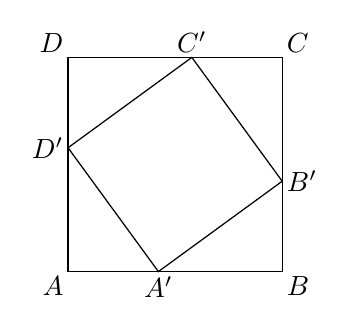
\begin{tikzpicture}[scale=0.85, line width=0.45pt,
  every node/.style={inner sep=1.5pt}]
  \coordinate (A) at (0,0);
  \coordinate (B) at (3.2,0);
  \coordinate (C) at (3.2,3.2);
  \coordinate (D) at (0,3.2);
  \coordinate (Ap) at (1.35,0);
  \coordinate (Bp) at (3.2,1.35);
  \coordinate (Cp) at (1.85,3.2);
  \coordinate (Dp) at (0,1.85);
  \draw (A)--(B)--(C)--(D)--cycle;
  \draw (Ap)--(Bp)--(Cp)--(Dp)--cycle;
  \node[anchor=north east] at (A) {$A$};
  \node[anchor=north west] at (B) {$B$};
  \node[anchor=south west] at (C) {$C$};
  \node[anchor=south east] at (D) {$D$};
  \node[anchor=north] at (Ap) {$A'$};
  \node[anchor=west] at (Bp) {$B'$};
  \node[anchor=south] at (Cp) {$C'$};
  \node[anchor=east] at (Dp) {$D'$};
\end{tikzpicture}
